% Lab 10 on Recursion
%
% CSE/IT 107: Introduction to Programming
% New Mexico Tech
%
\documentclass[11pt]{cselabheader}

%%%%%%%%%%%%%%%%%% SET TITLES %%%%%%%%%%%%%%%%%%%%%%%%%
\fancyhead[R]{Lab 10: Recursion}
\title{Lab 10: Recursion}

\begin{document}

\maketitle
\pagenumbering{roman}
\hrule

\begin{quote}
``A mirror mirroring a mirror.''

``In the end, we self-perceiving, self-inventing, locked-in mirages
are little miracles of self-reference.''
\end{quote}
\begin{flushright}
--- Douglas R. Hofstadter, I Am a Strange Loop
\end{flushright}

\hrule

\begin{figure}[H]
  \centering
  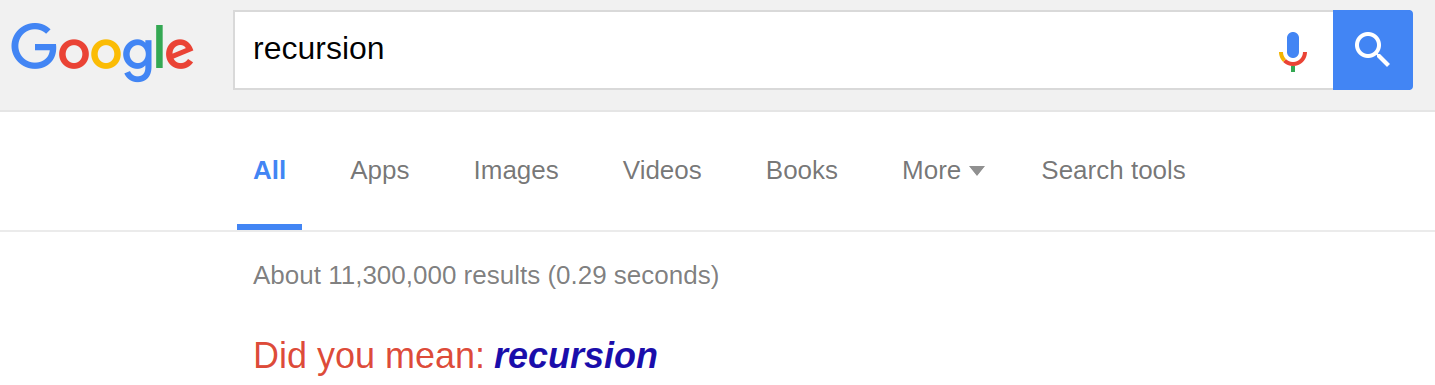
\includegraphics[width=\textwidth]{img/didyoumean.png}
  \caption{Google search for recursion (2016).}
\end{figure}

\begin{figure}[H]
  \centering
  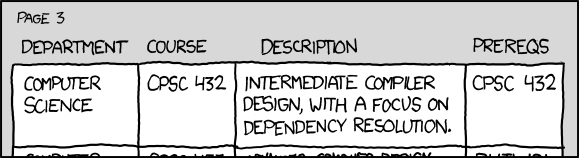
\includegraphics[width=0.5\textwidth]{img/xkcd_dependencies.png}
  \caption{Dependencies \url{http://xkcd.com/754/}}
\end{figure}

\hrule

\pagebreak
\tableofcontents

\section*{Introduction}
\addcontentsline{toc}{section}{Introduction}

\pagebreak
\pagenumbering{arabic}

how else can we repeat things? traverse a data structure?

\section{A Function Can Call Itself}
\subsection{Functions}
copy and paste function body

\subsection{Recursion}

what about this function?

\begin{python3code}
def count(n):
    print(n)
    count(n - 1)
\end{python3code}

If we call this function, the code will not stop.
It is the same as this loop:

copy and paste with \dots

but it does not terminate!

to print, you must print; how to print? print!

example:
how do you do 5 homework problems?
do the first one and then do 4 homework problems

how do you do 4 homework problems?
do the first one and then do 3 homework problems

...

how do you do 1 homework problems
do the problem then you're done

this can be generalized:

\subsection{Examples with One Recursive Call}
\subsubsection{Traversing Data}
describe
\begin{python3code}
def find_after_index(elem, current_index, elems):
    if current_index >= len(elems):
        return -1
    if elems[current_index] == elem:
        return current_index
    else:
        return find_after_index(elem, current_index + 1, elems)
\end{python3code}

that code is equivalent to

\begin{python3code}
\end{python3code}

step by step example

let's walk through it
(call stack)

translate a for loop to recursive calls

\begin{python3code}

\end{python3code}

\begin{python3code}

\end{python3code}

\subsubsection{Creating Data}
newton's method: guess sqrt

\begin{python3code}

\end{python3code}

factorial

\begin{python3code}

\end{python3code}

draw spiral

\begin{python3code}

\end{python3code}

\subsection{Examples with Multiple Recursive Calls}
\subsubsection{Creating Data}
draw tree

\begin{python3code}

\end{python3code}

\subsubsection{Traversing Data}
sum lists

\begin{python3code}

\end{python3code}

\subsection{Components of a Recursive Function}
base case, one or more recursive calls

``real world'' uses; why not loops, when to use
when size is being reduced
or
when traversing hierarchical data structures,
used in DE solutions, parsing code

can be easier to read, can be harder to predict

In a natural language, write down how a solution to your problem could be built from a solution to the same problem for a smaller input.

\newpage
\section{Exercises}

\begin{ex}[palindrome.py]
\end{ex}

\begin{ex}[list\_function.py]
\end{ex}

\begin{ex}[cesaro.py]
\end{ex}

\section{Extra Credit Exercises}

\begin{extraex}[lsystem.py]
\end{extraex}

\begin{infobox}{Supplementary Files}
\end{infobox}

\newpage
\section{Submitting}

You should submit your code as a tarball. It should contain all files
used in the exercises for this lab. The submitted file should be named
\begin{center}
  \texttt{cse107\_firstname\_lastname\_lab10.tar.gz}
\end{center}

\begin{center}
  \textbf{Upload your tarball to Canvas.}
\end{center}

\listofexercises
\listofextraexercises

\end{document}
